%
% FH Technikum Vienna
% !TEX encoding = UTF-8 Unicode
%
% Creation of Master and Bachelor theses at the FH Technikum Wien using LaTeX and the TWBOOK class
%
% To create your own document you have to add the following:
% 1) Set[...] with \documentclass: Master's or Bachelor's thesis, course of study and language.
% 2) With \newcommand{\FHTWCitationType}. Set citation standard (is usually given by the study program - please ask)
% 3) fill in cover sheet, abstract, etc.
% 4) and write the paper (enter the used literature sources in Literatur.bib)
%
% Tested with TeXstudio with character encoding ISO-8859-1 (=ansinew/latin1) and MikTex under Windows
% Note that the encoding of the file matches the encoding of the package inputenc!
% The encoding of the file twbook.cls MUST be ANSI!
% When using UTF8 not only the encoding of the document must be set to UTF8, but also the encoding of the BibTex file!
%
% Please send bugreports and feedback via email to latex@technikum-wien.at
%
% Versions
% *) V0.7: 9.1.2015, RO: modeline adjusted and moved
% *) V0.6: 10.10.2014, RO: Further adaptation to UK
% *) V0.5: 8.8.2014, WK: Literature sources revised and adapted
% *) V0.4: 4.8.2014, WK: Inital version imported into SVN
%
\documentclass[MSE,Master,english]{twbook}%\documentclass[Bachelor,BMR,ngerman]{twbook}
\usepackage[utf8]{inputenc}
\usepackage[T1]{fontenc}
\usepackage{float}
\usepackage{csquotes}
\usepackage{multicol}
\usepackage{graphicx}
\graphicspath{ {./PICs/} }

\tolerance=1
\emergencystretch=\maxdimen
\hyphenpenalty=10000
\hbadness=10000

%
% Hier biblatex & Biber konfigurieren; Vergessen Sie nicht, dass Sie biber verwenden müssen um eine Bibliothek zu erzeugen
%
\usepackage[backend=biber, style=numeric]{biblatex}
\addbibresource{Literatur.bib}

%
% Bei Bedarf bitte hier die Syntax-Highlightings anpassen
%
\usepackage[final]{listings}
\lstset{captionpos=b, numberbychapter=false,caption=\lstname,frame=single, numbers=left, stepnumber=1, numbersep=2pt, xleftmargin=15pt, framexleftmargin=15pt, numberstyle=\tiny, tabsize=3, columns=fixed, basicstyle={\fontfamily{pcr}\selectfont\footnotesize}, keywordstyle=\bfseries, commentstyle={\color[gray]{0.33}\itshape}, stringstyle=\color[gray]{0.25}, breaklines, breakatwhitespace, breakautoindent}
\lstloadlanguages{[ANSI]C, C++, [gnu]make, gnuplot, Matlab}

\usepackage[xindy]{glossaries}
\makenoidxglossaries
\renewcommand{\glossarysection}[2][]{}
%Formatieren des Quellcodeverzeichnisses
\makeatletter
% Setzen der Bezeichnungen für das Quellcodeverzeichnis/Abkürzungsverzeichnis in Abhängigkeit von der eingestellten Sprache
\providecommand\listacroname{}
\@ifclasswith{twbook}{english}
{%
    \renewcommand\lstlistingname{Code}
    \renewcommand\lstlistlistingname{List of Code}
    \renewcommand\listacroname{List of Abbreviations}
}{%
    \renewcommand\lstlistingname{Quellcode}
    \renewcommand\lstlistlistingname{Quellcodeverzeichnis}
    \renewcommand\listacroname{Abkürzungsverzeichnis}
}
% Wenn die Option listof=entryprefix gewählt wurde, Definition des Entyprefixes für das Quellcodeverzeichnis. Definition des Macros listoflolentryname analog zu listoflofentryname und listoflotentryname der KOMA-Klasse
\@ifclasswith{scrbook}{listof=entryprefix}
{%
    \newcommand\listoflolentryname\lstlistingname
}{%
}
\makeatother
\newcommand{\listofcode}{\phantomsection\lstlistoflistings}

% Die nachfolgenden Pakete stellen sonst nicht benötigte Features zur Verfügung
\usepackage{blindtext}
%
% Einträge für Deckblatt, Kurzfassung, etc.
%
\title{Transparency in\\Decentraland DAO}
\author{Comerci Wolcanyik, Nicol{\'a}s}
\studentnumber{2120299002}
%\author{Titel Vorname Name, Titel\and{}Titel Vorname Name, Titel}
%\studentnumber{XXXXXXXXXXXXXXX\and{}XXXXXXXXXXXXXXX}
\supervisor{Dinhof, Gerhard}
%\supervisor[Begutachter]{Titel Vorname Name, Titel}
%\supervisor[Begutachterin]{Titel Vorname Name, Titel}
%\secondsupervisor{Titel Vorname Name, Titel}
%\secondsupervisor[Begutachter]{Titel Vorname Name, Titel}
%\secondsupervisor[Begutachterinnen]{Titel Vorname Name, Titel}
\place{Vienna}
\outline{\toComplete}
\keywords{Keyword1, Keyword2, Keyword3, Keyword4}
\acknowledgements{\toComplete}

% Glossary entries
\newglossaryentry{MANA}
{
  name=MANA,
  description={Is Decentraland's fungible, ERC20 cryptocurrency token limited to a total original supply of 2,805,886,393},
}
\newglossaryentry{LAND}
{
  name=LAND,
  description={Is a scarce, non-fungible digital asset maintained in an Ethereum smart contract that represents the parcels of virtual land within Decentraland},
  plural=LANDs
}
\newglossaryentry{ESTATE}
{
  name=ESTATE,
  description={A cluster of adjacent LANDs},
  plural=ESTATEs
}
\newglossaryentry{NFT}
{
  name=NFT,
  description={non-fungible tokens are unique, distinguishable digital assets. The information contained within a non-fungible token is unique to that token},
  plural=NFTs
}

\begin{document}
\maketitle

%
% .. und hier beginnt die eigentliche Arbeit. Viel Erfolg beim Verfassen!
%
\chapter{Introduction}
From October 31, 2008 (when the Bitcoin whitepaper was published) to the present day, people's interest in Blockchain technology has been growing progressively and increased exponentially from 2020 onwards. 

There are a large number of projects that rely on this technology to date, one of them is Decentraland: a 3D digital world that will be discussed in the next section and that uses Ethereum to execute its transactions.

One of the great advantages of Blockchain is transparency: anyone can verify all transactions made, from the first to the last. But how easy is it for an average user to access this information? What kind of analysis and conclusions can be drawn once obtained? This paper will seek to answer these questions specifically using Decentraland's DAO as the object of study. \\
\toComplete
\clearpage

\chapter{Basics}
\section{Blockchain}
Today there are different types of blockchain, but based on the original concept and taking as a reference the article \emph{"La blockchain: fundamentos, aplicaciones y relaci{\'o}n con otras tecnolog{\'\i}as disruptivas"}\cite{blockchain}, it was created to store the transaction history of Bitcoin, but with the course of time it has seen great potential to be applied in other areas due to the properties it offers. The blockchain provides an immutable distributed database based on a growing sequence of blocks. These blocks, being public, form an open system that enhances trust based on the transparency and robustness of the blockchain construction technique. The system, although open, is also semi-anonymous: users identify themselves with public keys (pseudonyms), not with their real identities.

This database can be shared by a large number of users on a \emph{peer-to-peer} basis and allows information to be stored in an immutable and orderly manner. The information added to the blockchain is public, can be accessed at any time by any user of the network and can only be added to the blockchain if there is an agreement between the majority of the parties. After a certain period of time, it can be assumed that the information added to a block can no longer be modified (immutability).

By design, this system intrinsically provides tolerance to node failures, robustness against manipulation and transparency, since it is public.

\section{Digital Assets}
A digital asset\cite{digAssets} is generally anything that is created and stored digitally, is identifiable and discoverable, and has or provides value. Digital assets have become more popular and valuable as technological advances become integrated into our personal and professional lives. Data, images, video, written content, and more have long been considered digital assets with ownership rights.

Most digital items, like a company's brand, can be assigned a value, monetary or intangible. Some digital items might only be valuable to the creator or one person, such as a family picture on your phone taken at a gathering. Others could be valuable to a much wider audience.

In the past, digital assets such as data or scanned documents were owned and used by organizations to realize value. However, when blockchain and cryptocurrency were introduced in 2009, digital assets were again redefined. Anything in digital form became something that could be used to create value via tokenization on a blockchain. \\

\ac{Crypto} is essentially a digital currency that use blockchain technology and cryptography to facilitate secure and anonymous transactions. The crypto market is worth over USD 500 billion.\cite{crypto}

\begin{figure}[H]
  \centering
  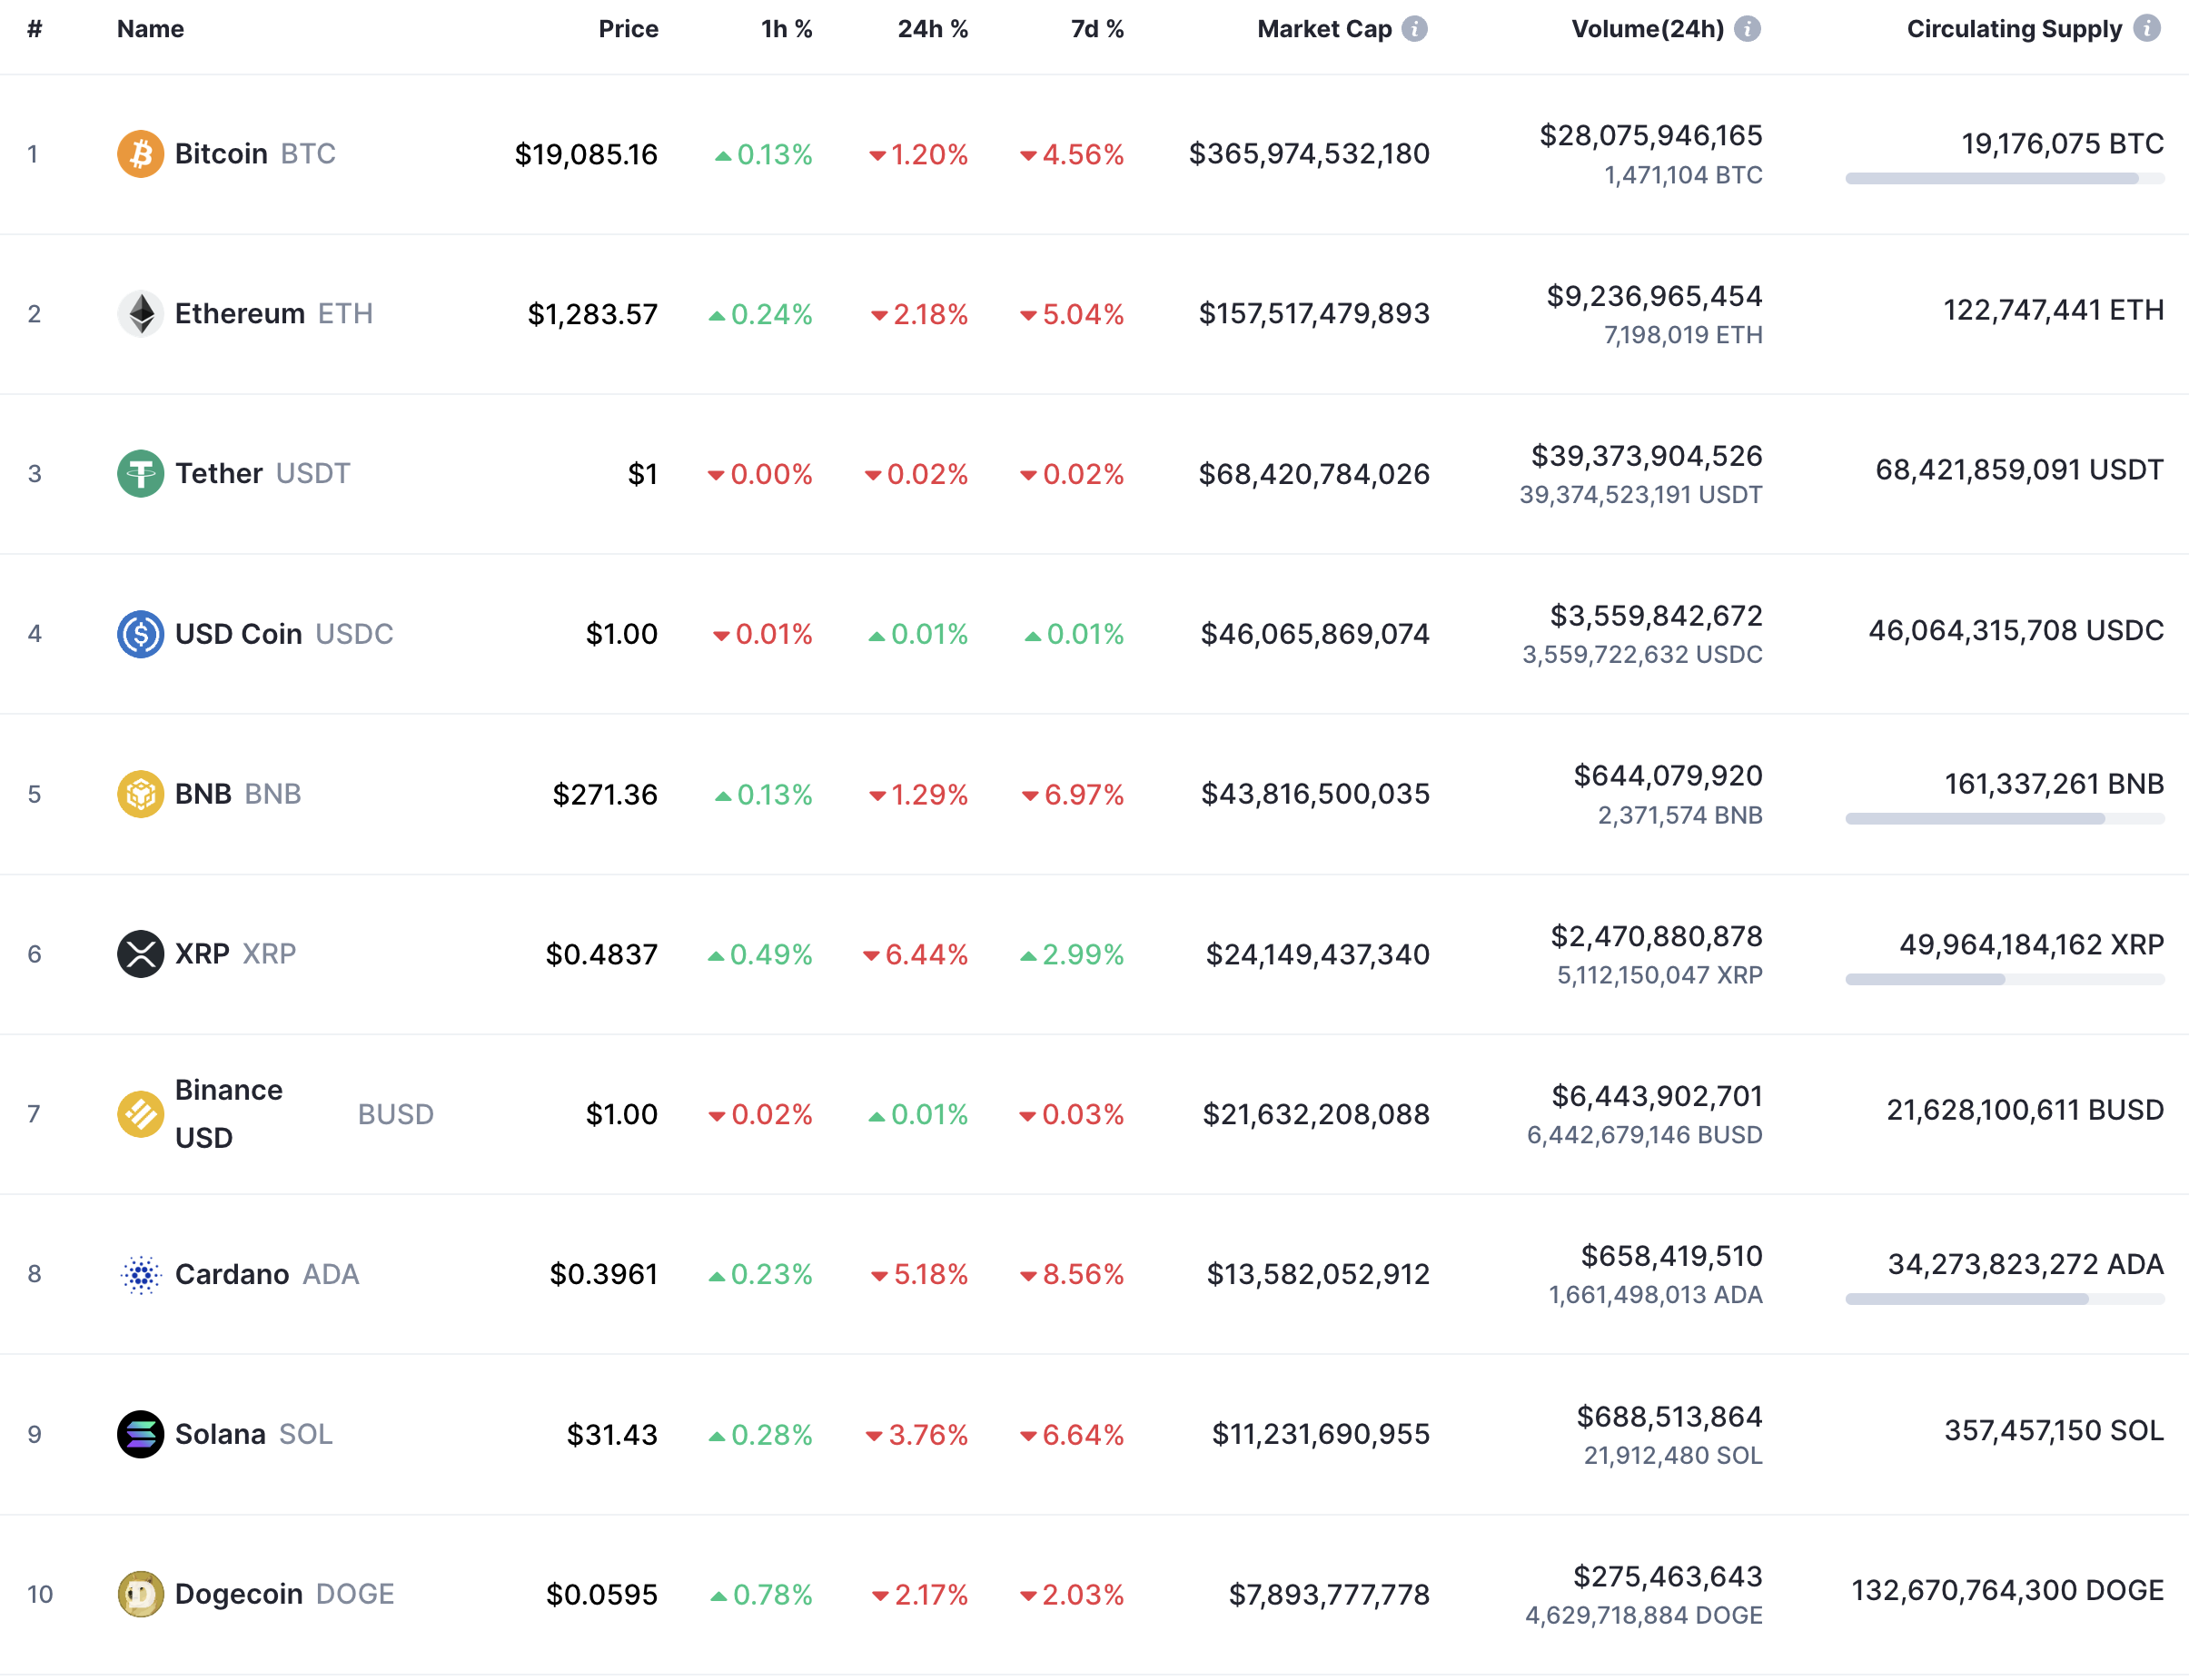
\includegraphics[width=\textwidth]{crypto_ranking.png}
  \caption{Top 10 cryptocurrencies by market capitalization \cite{coinmarketcap}}
  \label{fig:ranking}
\end{figure}

What made it different from normal bank transfers or other financial services like Paypal is that there was no middle man for the first time. A middle-man is a central authority like a bank or government that intervenes in a transaction between the sender and recipient. They have the power to surveill, censor or revert transactions and they can share the sensitive data they collect with third parties. They also often dictate which financial services people have access to.\cite{ethereum} \\

There are many different types of digital assets.\cite{digAssets} Here is a list of many of the familiar ones:
\begin{multicols}{2}
  \begin{itemize}
    \item Photos
    \item Documents
    \item Videos
    \item Books
    \item Audio/Music
    \item Animations
    \item Illustrations
    \item Manuscripts
    \item Emails and email accounts
    \item Logos
    \item Metadata
    \item Content
    \item Social media accounts
    \item Gaming accounts
  \end{itemize}
\end{multicols}

Newer digital assets are based on blockchain or similar technologies:
\begin{multicols}{2}
  \begin{itemize}
    \item Non-Fungible Tokens
    \item Cryptocurrency
    \item Tokens
    \item Crypto Assets
    \item Tokenized Assets
    \item Security Tokens
    \item Central Bank Digital Currencies
  \end{itemize}
\end{multicols}

It is worth devoting a few paragraphs to the Non-Fungible Tokens (\glspl{NFT}): for the purposes of definition, a non-fungible token\cite{nft} can be seen as a unit of digital information (token) that is stored on a blockchain and is not inherently interchangeable with other digital assets (non-fungible). The term "fungible" derives from the economic and accounting literatures, and is defined as anything that is interchangeable with an identical or similar object. Traditional form of currency, whether equivalent sums of paper money or identical unit of precious metals, are fungible objects, and this is what helps them to serve as mediums of exchange, because they are understood to be of equal value. One can substitute a five-dollar bill with five one-dollar bills because both are fungible.

Assets that are commonly considered fungible are regulated commodities, common shares (stocks), financial options, and bills of money. By contrast, a non-fungible asset may be a person's car, for example, since someone borrowing a friend's car would not repay their debt to their friend by giving them another person's car. Collectible items such as baseball cards represent a traditional example of non-fungible assets, since each card would have unique attributes which enhance or diminish their value compared to other baseball cards. In the virtual realm, objects were originally thought to be difficult in terms of proving their uniqueness and distinguishability so that they could be considered "non-fungible".

\section{Smart contracts\label{sm}}
\emph{"A smart contract is a computerized transaction protocol that executes the terms of a contract. The general objectives of smart contract design are to satisfy common contractual conditions (such as payment terms, liens, confidentiality, and even enforcement), minimize exceptions both malicious and accidental, and minimize the need for trusted intermediaries. Related economic goals include lowering fraud loss, arbitration and enforcement costs, and other transaction costs."} Nick Szabo, 1994.\cite{smartContracts} \\

Smart contracts live on the Ethereum blockchain  (see \ref{eth}). They only execute when triggered by a transaction from a user (or another contract). These programs are called \ac{Dapp}.

Once a smart contract is published to Ethereum, it will be online and operational for as long as Ethereum exists. Not even the author can take it down. Since smart contracts are automated, they do not discriminate against any user and are always ready to use.\cite{ethereum}

\section{Ethereum\label{eth}}
Ethereum is a technology for building apps and organizations, holding assets, transacting and communicating without being controlled by a central authority. There is no need to hand over personal details to use it - the user remains in control of their own data and what is being shared. Ethereum has its own cryptocurrency, Ether, which is used to pay for certain activities on the Ethereum network.

Also it is \textbf{programmable} using \textbf{smart contracts}, so that means that people can build apps that use the blockchain to store data or control what apps can do. This results in a general purpose blockchain that can be programmed to do anything.\cite{ethereum}

\subsection{How did it begin?}
Although the Ethereum blockchain has a number of founders, Vitalik Buterin\cite{ethHistory} was the one who initially published a white paper explaining the concept of Ethereum in November 2013. Following Buterin's initial work, other brains jumped on board in various capacities to help bring the project to fruition.

It gained awareness in early 2014 when Buterin brought the concept of the blockchain project into the public eye at a Bitcoin conference in Miami Florida. The project raised capital via an initial coin offering (ICO) later the same year, selling millions of dollars worth of ETH coins in exchange for funds to use for the development of the project. Between July 22 and Sept. 2, 2014, the asset sale sold over \$18 million worth of ETH, paid for in Bitcoin.

Although ETH coins were purchasable in 2014, the Ethereum blockchain did not actually go live until July 30, 2015, meaning ETH buyers had to wait for the blockchain to launch before they could move or use their ETH. 

Called Frontier, the first iteration of the Ethereum blockchain simply got the chain off the ground and running, hosting smart contracts and proof-of-work mining. The initial launch gave folks the opportunity to set up their mining apparatuses and start building on the network.

\subsection{Proof-of-Work (PoW) vs. Proof-of-Stake (PoS)}
The Ethereum network began by using a consensus mechanism that involved \ac{PoW}\cite{PoW}. This allowed the nodes of the Ethereum network to agree on the state of all information recorded on the Ethereum blockchain and prevented certain kinds of economic attacks. However, Ethereum switched off proof-of-work in 2022 and started using proof-of-stake instead.

Proof-of-work is the underlying algorithm that sets the difficulty and rules for the work miners do on proof-of-work blockchains. Mining is the "work" itself. It's the act of adding valid blocks to the chain. This is important because the chain's length helps the network follow the correct fork of the blockchain. The more "work" done, the longer the chain, and the higher the block number, the more certain the network can be of the current state of things. \\

On Sept. 15, 2022 Ethereum switched to \ac{PoS}\cite{PoS}. In proof-of-work, miners prove they have capital at risk by expending energy. Ethereum uses proof-of-stake, where validators explicitly stake capital in the form of ETH into a smart contract on Ethereum. This staked ETH then acts as collateral that can be destroyed if the validator behaves dishonestly or lazily. The validator is then responsible for checking that new blocks propagated over the network are valid and occasionally creating and propagating new blocks themselves. \\

Proof-of-stake comes with a number of improvements to the now-deprecated proof-of-work system:

\begin{itemize}
  \item Better energy efficiency - there is no need to use lots of energy on proof-of-work computations
  \item Lower barriers to entry, reduced hardware requirements - there is no need for elite hardware to stand a chance of creating new blocks
  \item Reduced centralization risk - proof-of-stake should lead to more nodes securing the network
  \item Because of the low energy requirement less ETH issuance is required to incentivize participation
  \item Economic penalties for misbehaviour make 51\% style attacks exponentially more costly for an attacker compared to proof-of-work
  \item The community can resort to social recovery of an honest chain if a 51\% attack were to overcome the crypto-economic defenses.
\end{itemize}

\subsection{Statistics}

In the figure \ref{fig:dailyTxs} can be observed that the daily amount of transactions ranges between 1M and 1.25M since late 2020, with a peak of 1.7M daily transactions in May 2021.
\begin{figure}[H]
  \centering
  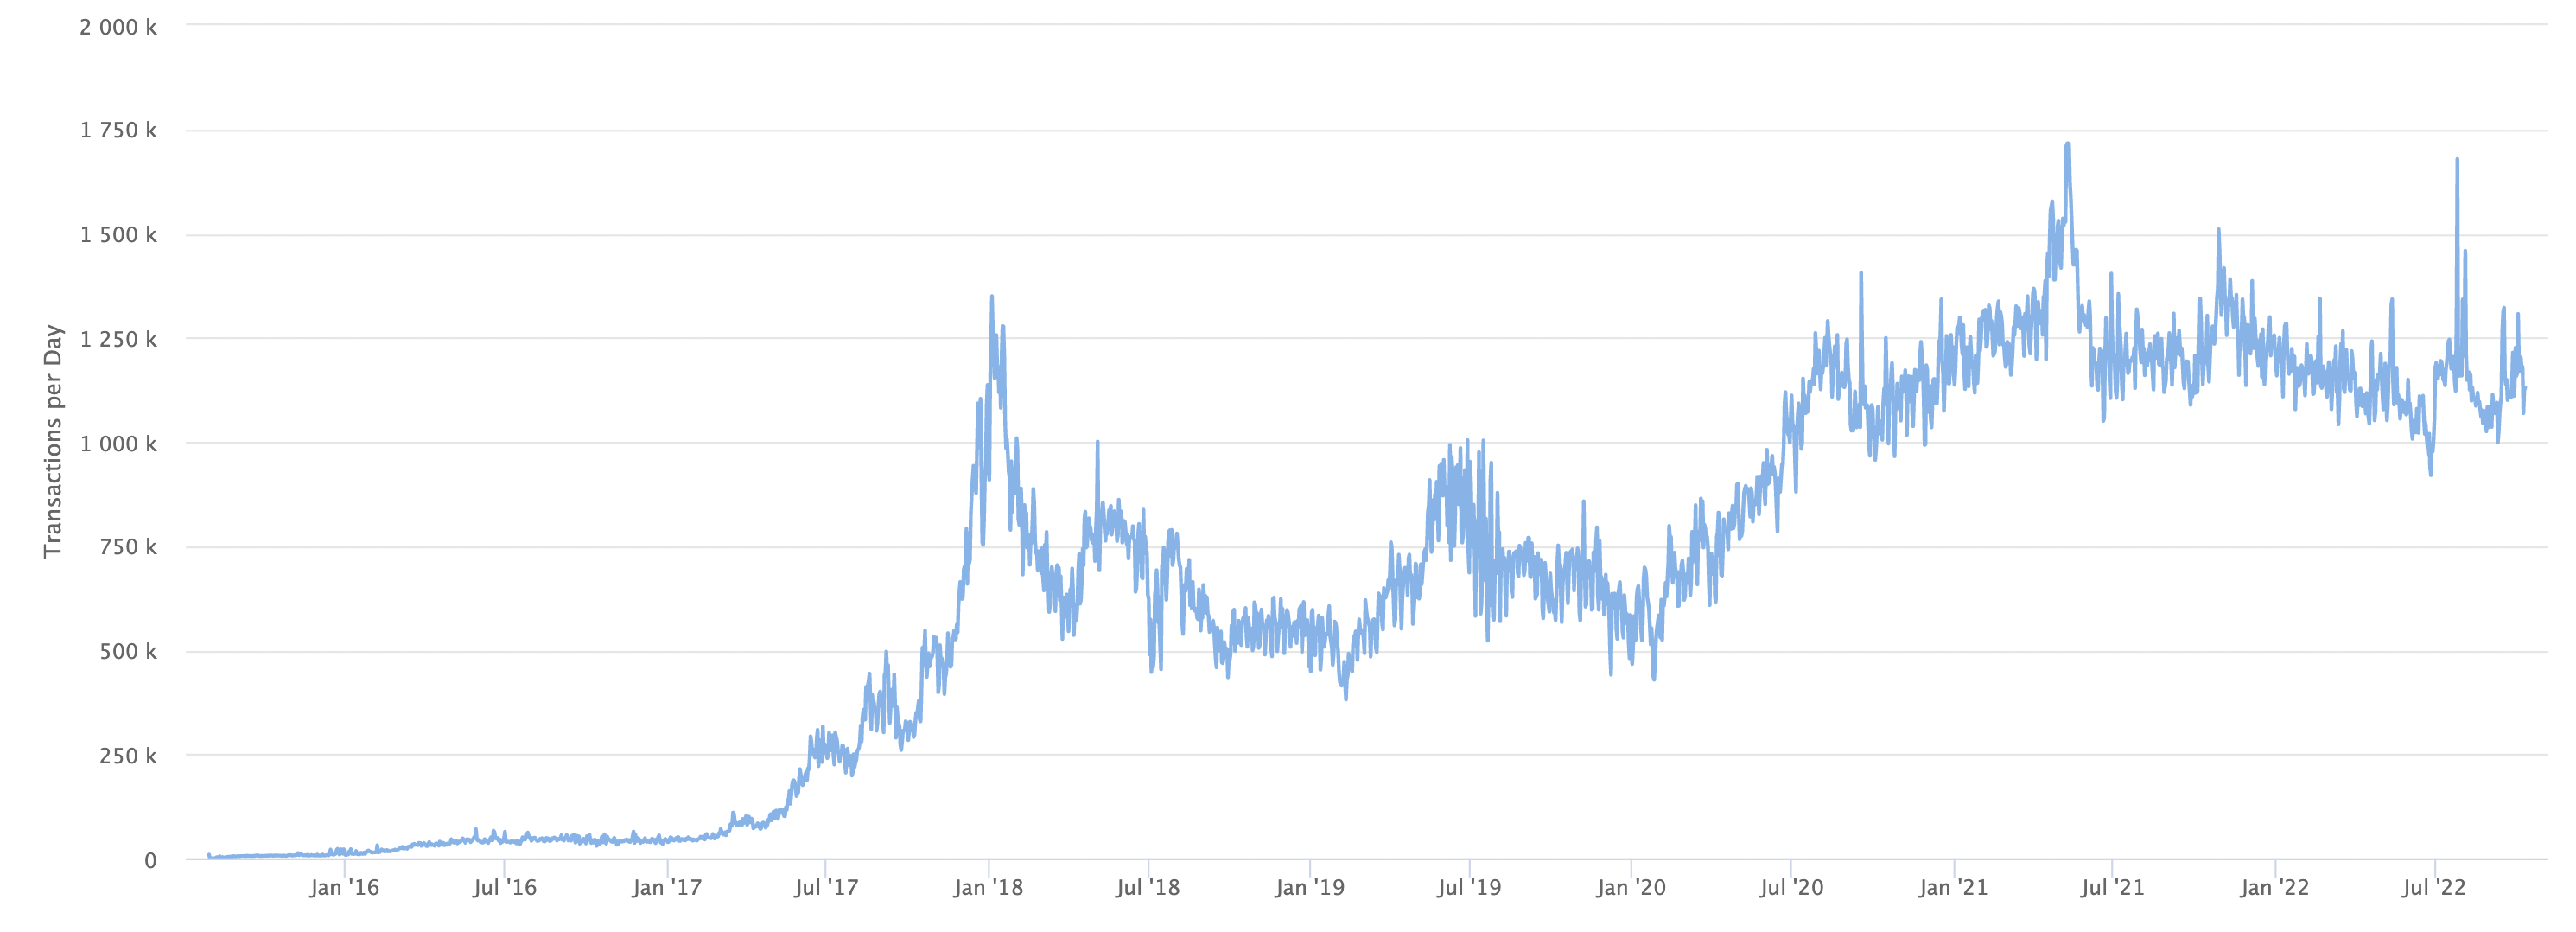
\includegraphics[width=\textwidth]{daily_txs.png}
  \caption{Daily Ethereum transactions \cite{etherscan}}
  \label{fig:dailyTxs}
\end{figure}

There are more than 200 million unique addresses in Ethereum as shown in the figure \ref{fig:uniqueAddr}.
\begin{figure}[H]
  \centering
  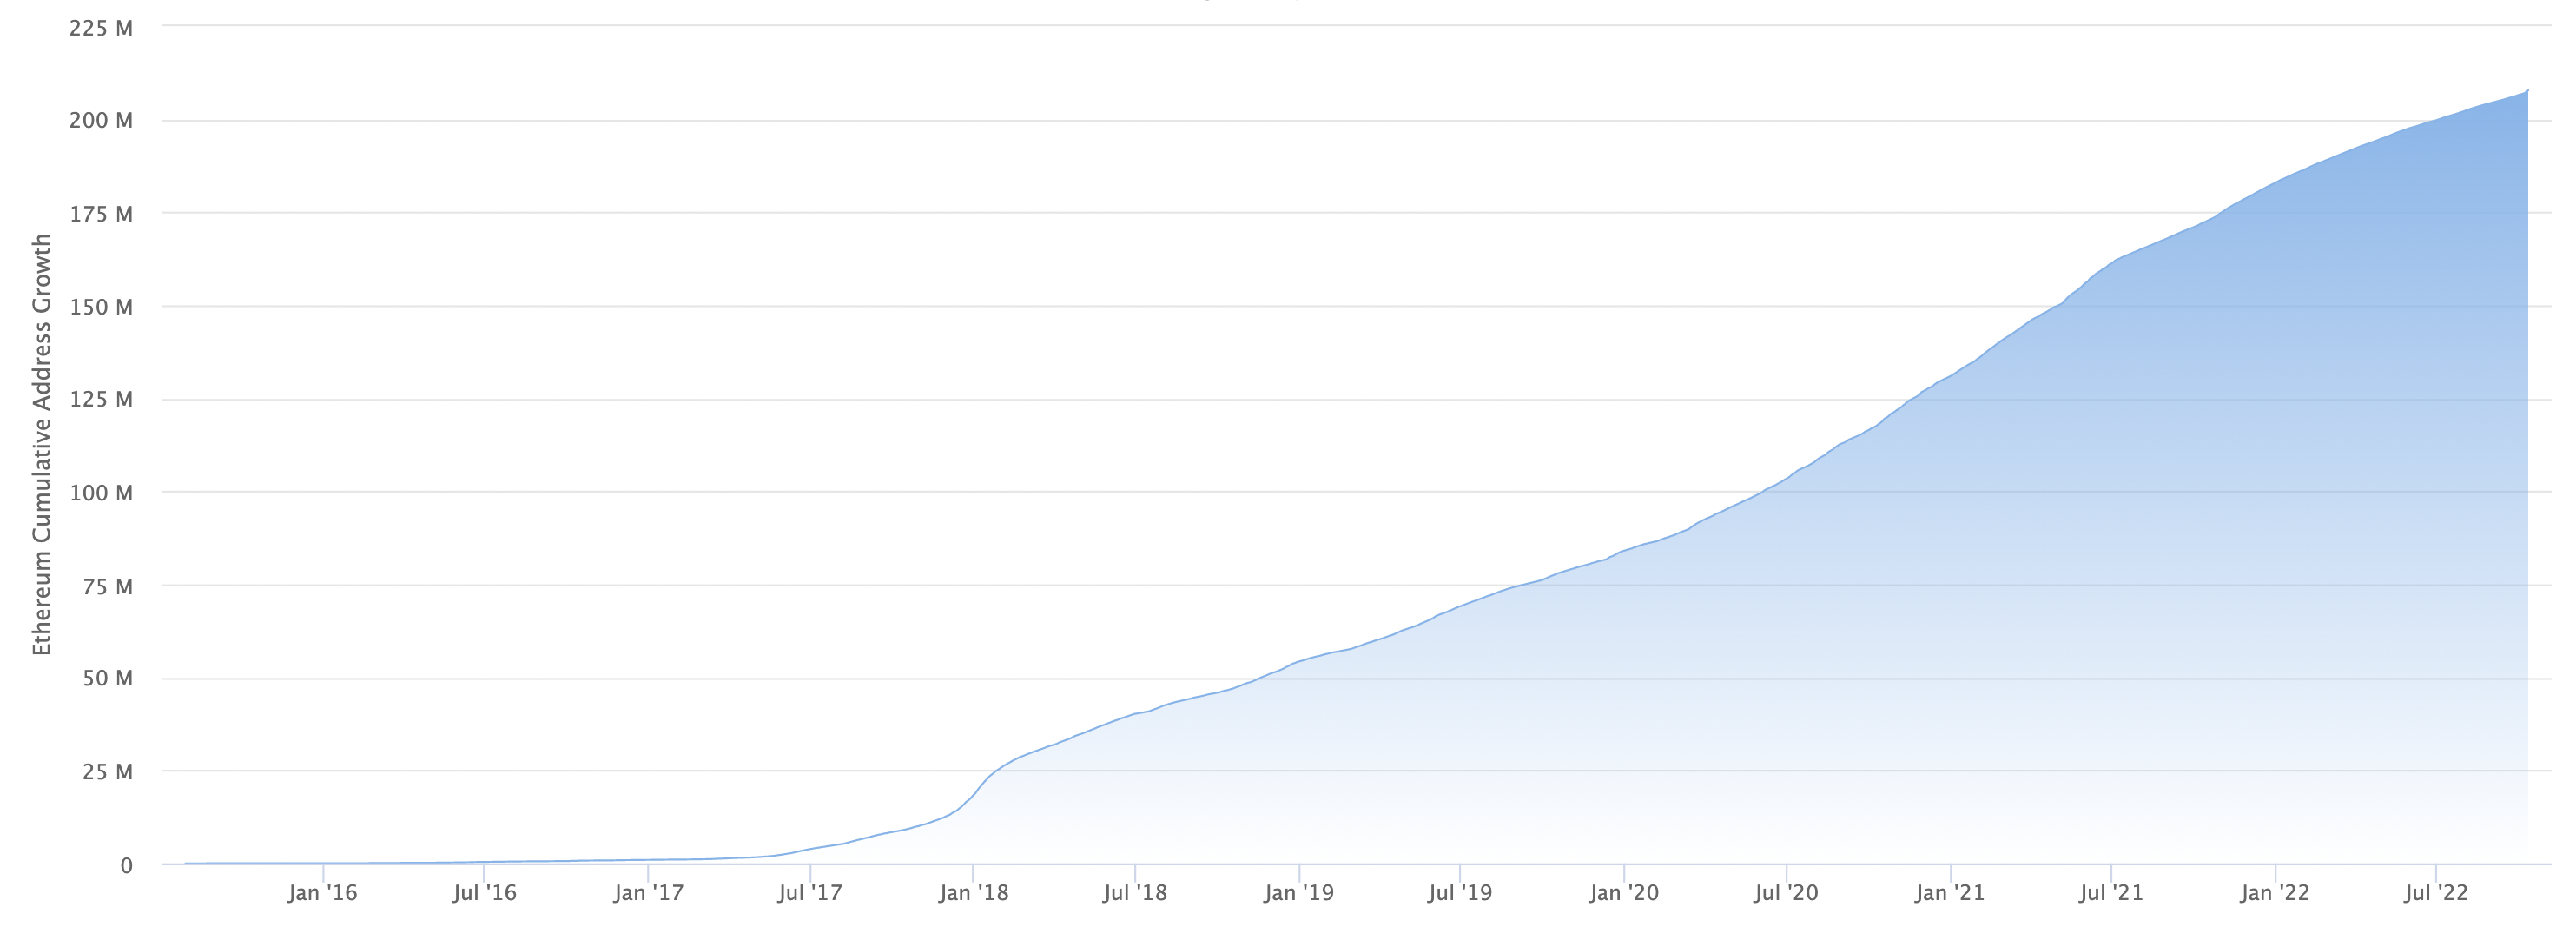
\includegraphics[width=\textwidth]{unique_addresses.png}
  \caption{Unique Ethereum addresses \cite{etherscan}}
  \label{fig:uniqueAddr}
\end{figure}

But only between 400,000 and 600,000 addresses are currently active, meaning between 0.2\% and 0.3\% of the unique addresses (see figure \ref{fig:activeAddr}).
\begin{figure}[H]
  \centering
  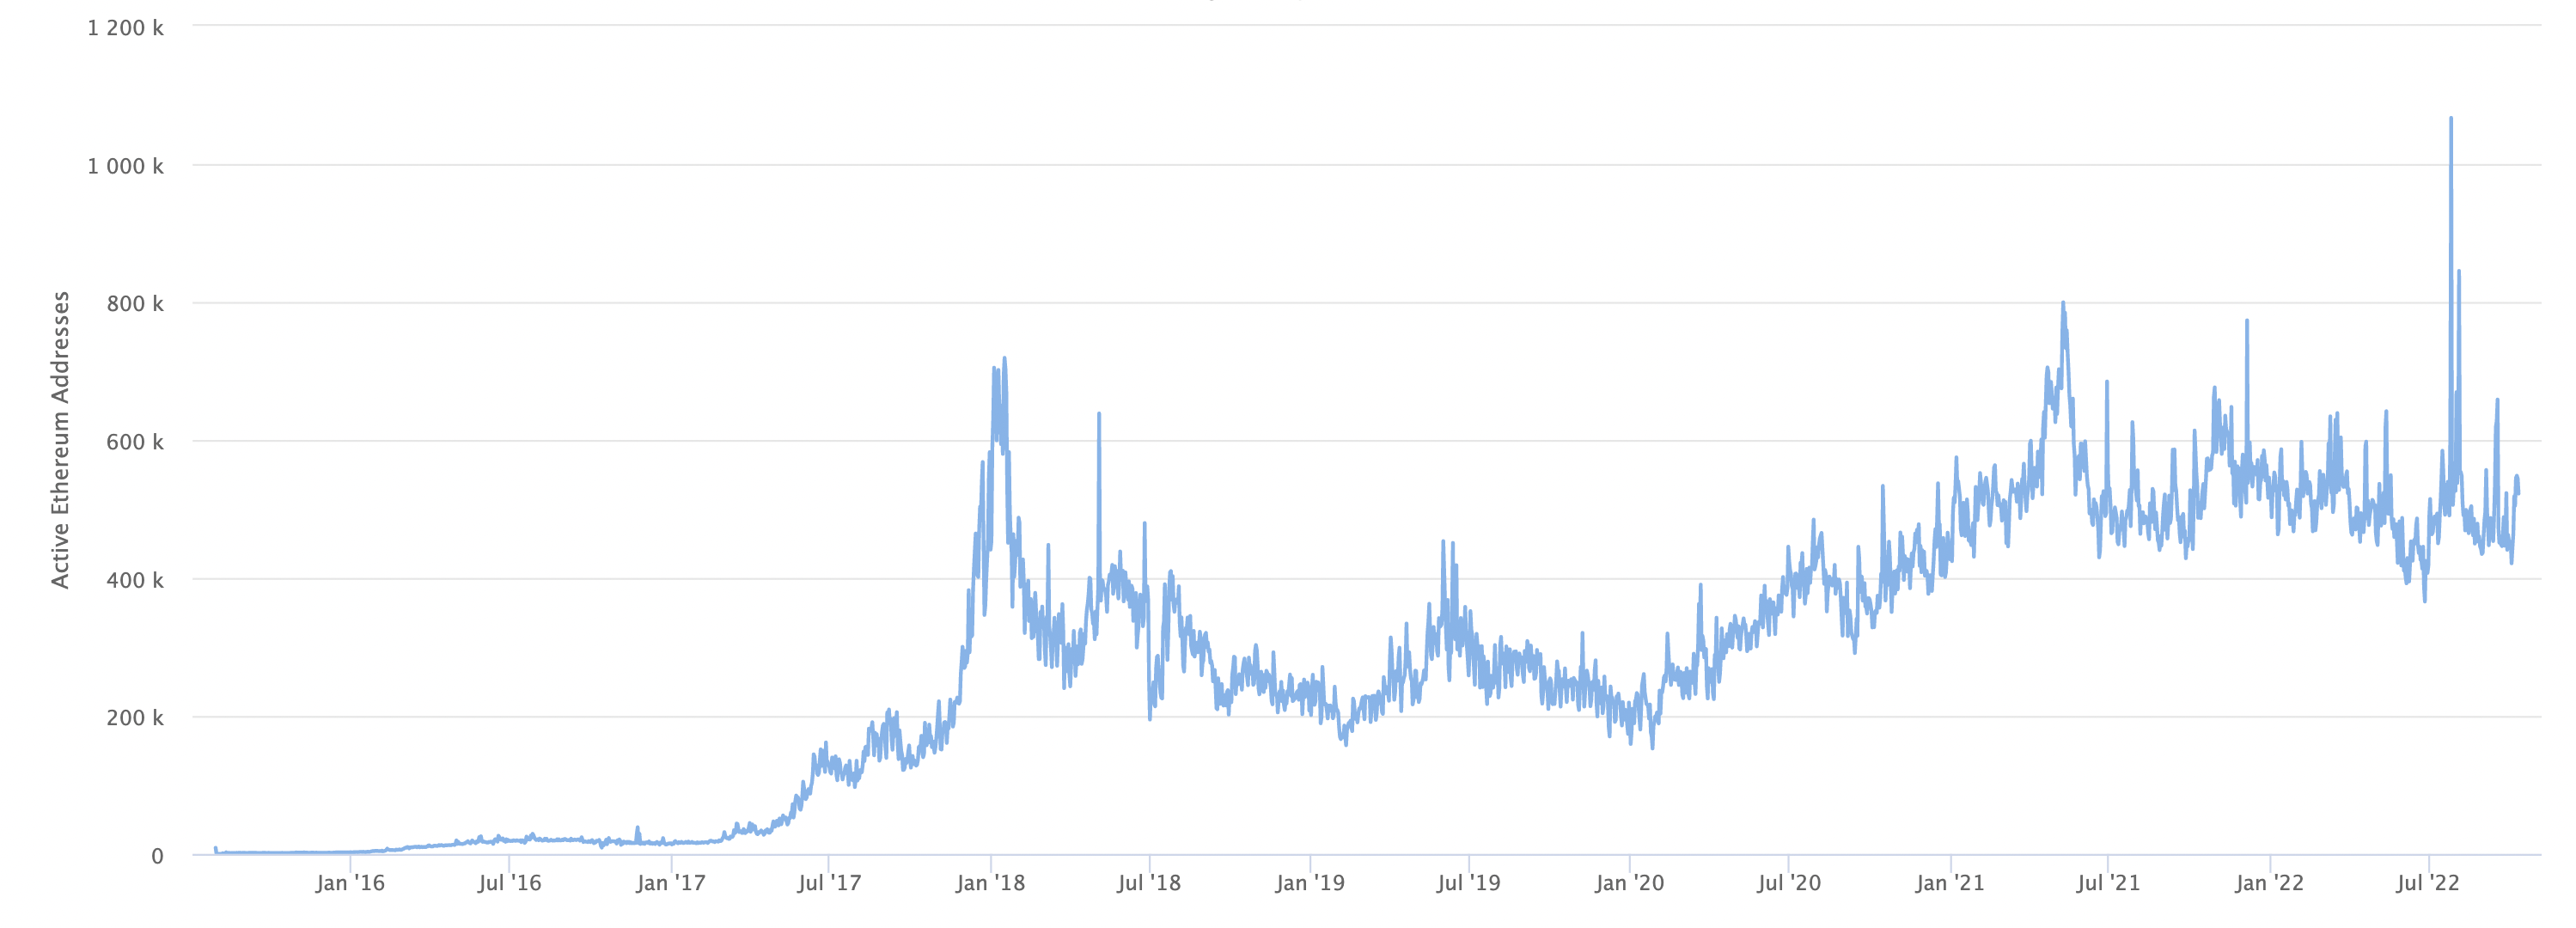
\includegraphics[width=\textwidth]{active_addresses.png}
  \caption{Active Ethereum addresses \cite{etherscan}}
  \label{fig:activeAddr}
\end{figure}

\section{\NoCaseChange{\acl{DAO}} (DAO)}
A DAO is a collectively-owned, blockchain-governed organization working towards a shared mission.

DAOs allow people to work with like-minded individuals around the globe without trusting a benevolent leader to manage the funds or operations. There is no CEO who can spend funds on a whim or CFO who can manipulate the books. Instead, blockchain-based rules baked into the code define how the organization works and how funds are spent.

They have built-in treasuries that no one has the authority to access without the approval of the group. Decisions are governed by proposals and voting to ensure everyone in the organization has a voice, and everything happens transparently on-chain.\cite{DAO} \\

Table \ref{table:DAOComparison} on page \pageref{table:DAOComparison} compares a DAO with a traditional organization:
\begin{center}
  \begin{table}[H]
    \begin{tabular}{ | m{20em} | m{20em} | }
      \hline
      \textbf{DAO} & \textbf{Traditional organization} \\ 
      \hline
      Usually flat, and fully democratized. & Usually hierarchical. \\
      \hline  
      Voting required by members for any changes to be implemented. & Depending on structure, changes can be demanded from a sole party, or voting may be offered. \\
      \hline
      Votes tallied, and outcome implemented automatically without trusted intermediary. & If voting allowed, votes are tallied internally, and outcome of voting must be handled manually. \\
      \hline
      Services offered are handled automatically in a decentralized manner (for example distribution of philanthropic funds). & Requires human handling, or centrally controlled automation, prone to manipulation. \\
      \hline
      All activity is transparent and fully public. & Activity is typically private, and limited to the public. \\
      \hline
    \end{tabular}
    \caption{Comparison between a DAO and a traditional organization \cite{DAO}}
    \label{table:DAOComparison}
  \end{table}
\end{center}

\section{Metaverse\label{dcl}}
\emph{"The Metaverse is the post-reality universe, a perpetual and persistent multiuser environment merging physical reality with digital virtuality. It is based on the convergence of technologies that enable multisensory interactions with virtual environments, digital objects and people such as \ac{VR} and \ac{AR}. Hence, the Metaverse is an interconnected web of social, networked immersive environments in persistent multiuser platforms. It enables seamless embodied user communication in real-time and dynamic interactions with digital artifacts. Its first iteration was a web of virtual worlds where avatars were able to teleport among them. The contemporary iteration of the Metaverse features social, immersive VR platforms compatible with massive multiplayer online video games, open game worlds and AR collaborative spaces."} Stylianos Mystakidis, 2022. \cite{metaverse} \\

\begin{figure}[H]
  \centering
  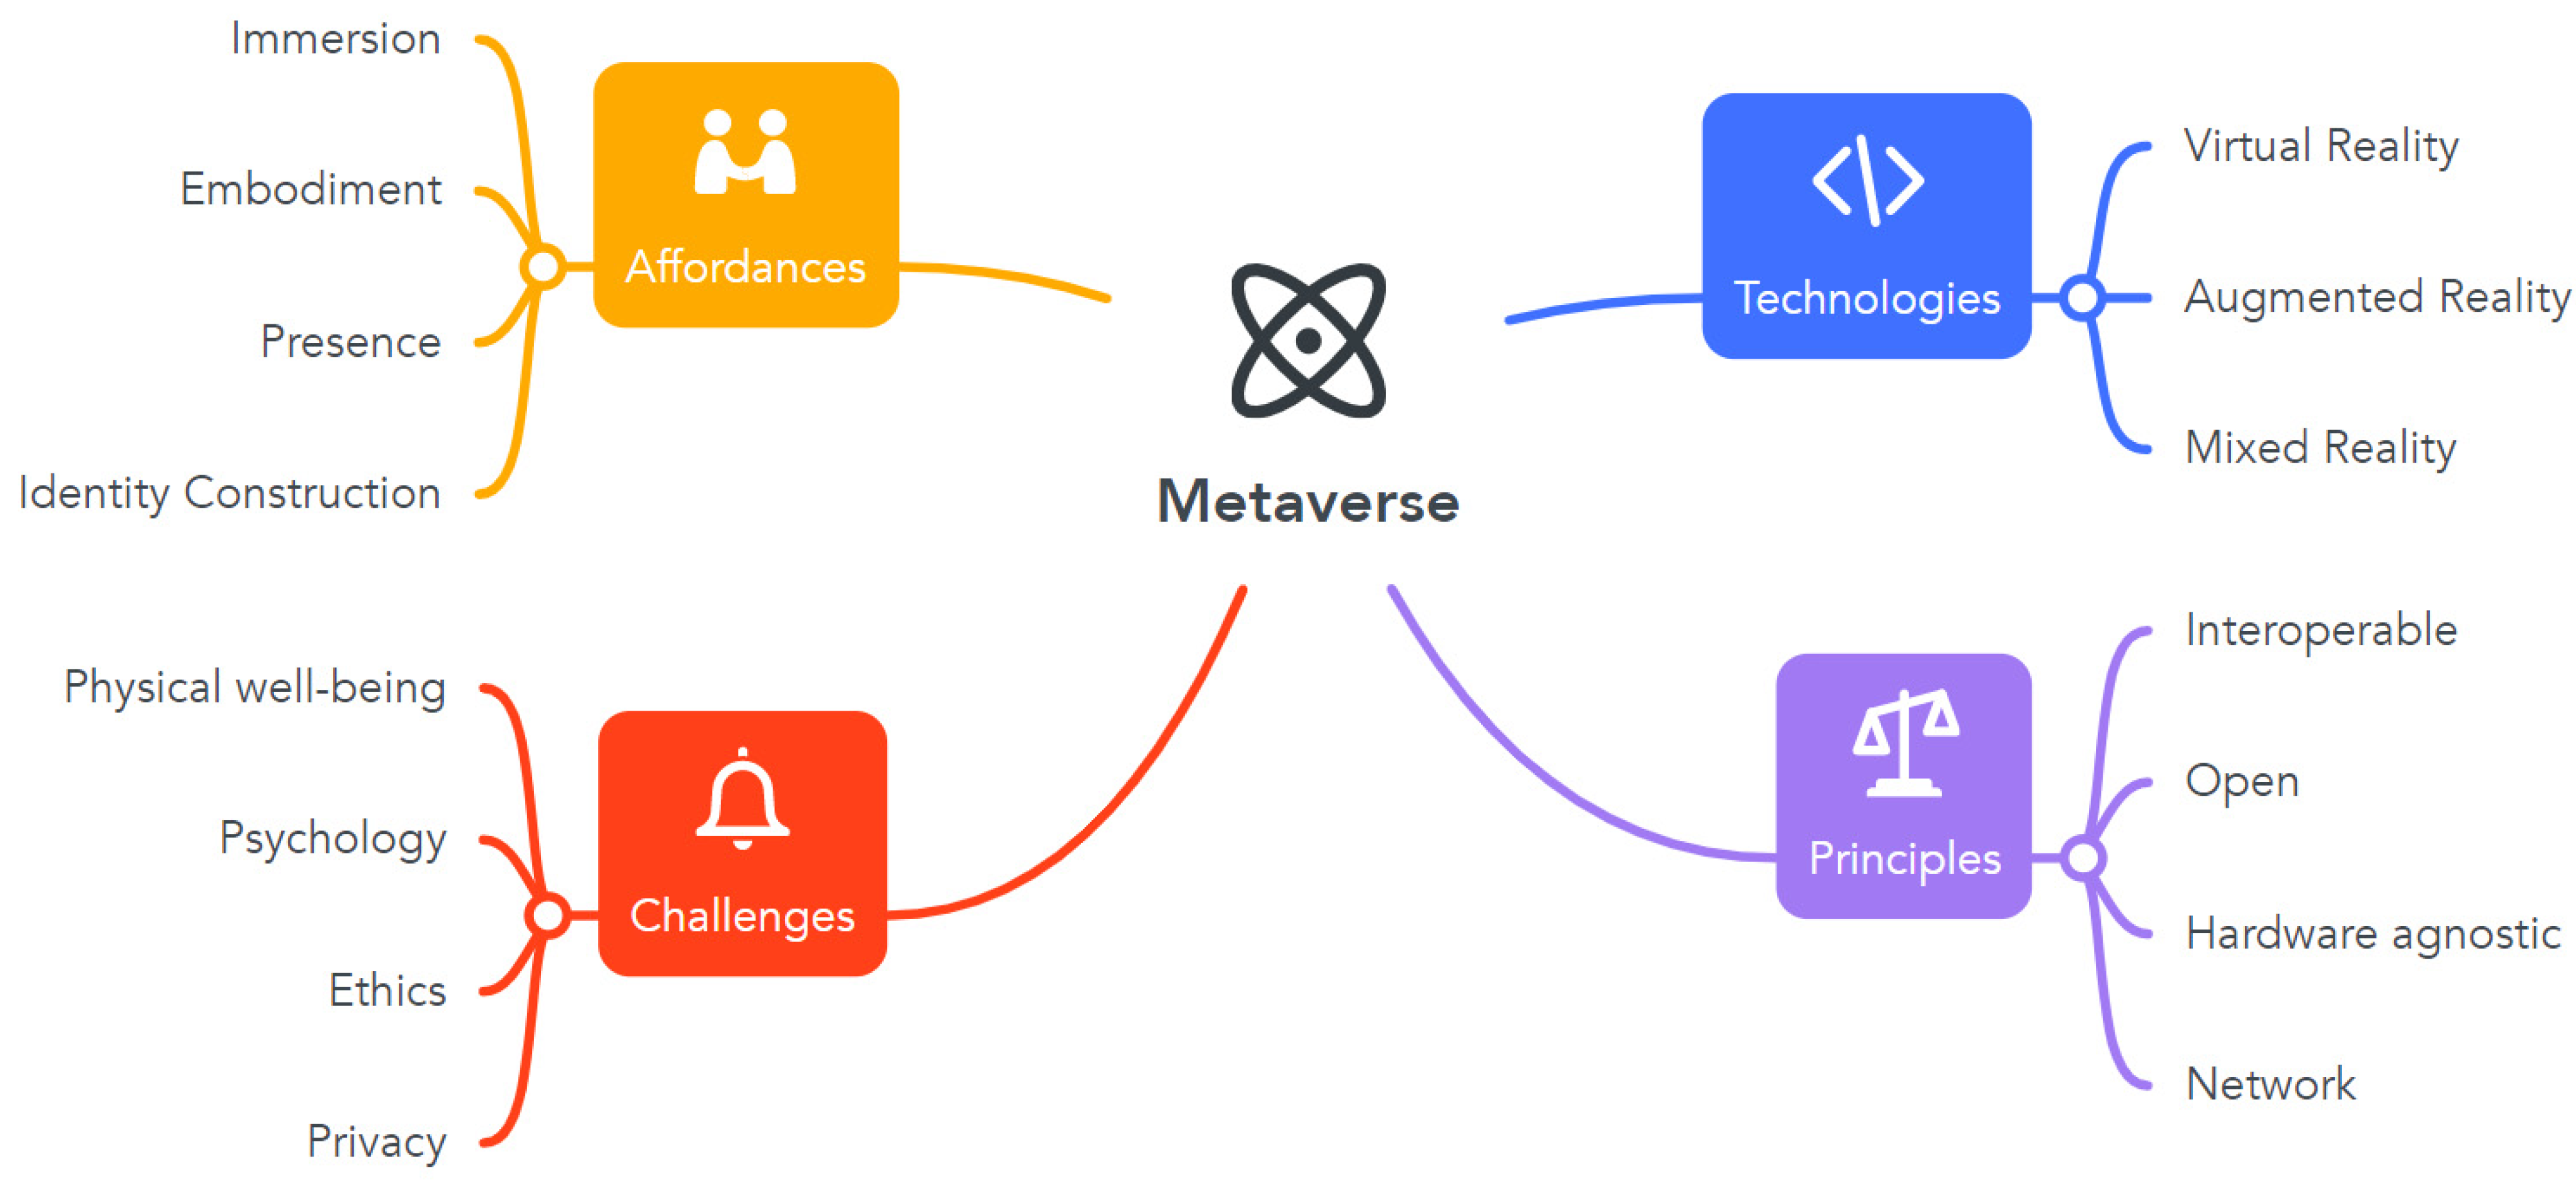
\includegraphics[width=\textwidth]{metaverse.png}
  \caption{Description of the metaverse \cite{metaverse}}
  \label{fig:metaverse}
\end{figure}

Decentraland\cite{DCL} is a decentralized virtual reality platform, better known as a metaverse, powered by the Ethereum blockchain. It is an open source project, maintained by the Decentraland Foundation and driven by its community. 

Within the Decentraland platform, users can create, experience, and monetize their content and applications. The finite, traversable, 3D virtual space within Decentraland is called \textbf{\gls{LAND}}, a non-fungible digital asset or more commonly known as a \ac{NFT}, maintained in an Ethereum smart contract. Land is divided into parcels that are identified by cartesian coordinates (x,y). These parcels are permanently owned by members of the community and are purchased using \textbf{\gls{MANA}}, Decentraland's cryptocurrency token. This gives users full control over the environments and applications that they create, which can range from anything like static 3D scenes to more interactive applications or games.

\begin{figure}[H]
  \centering
  
\includegraphics[width=\textwidth]{dcl.png}
  \caption{Screenshot of Decentraland}
  \label{fig:dcl}
\end{figure}

\begin{figure}[H]
  \centering
  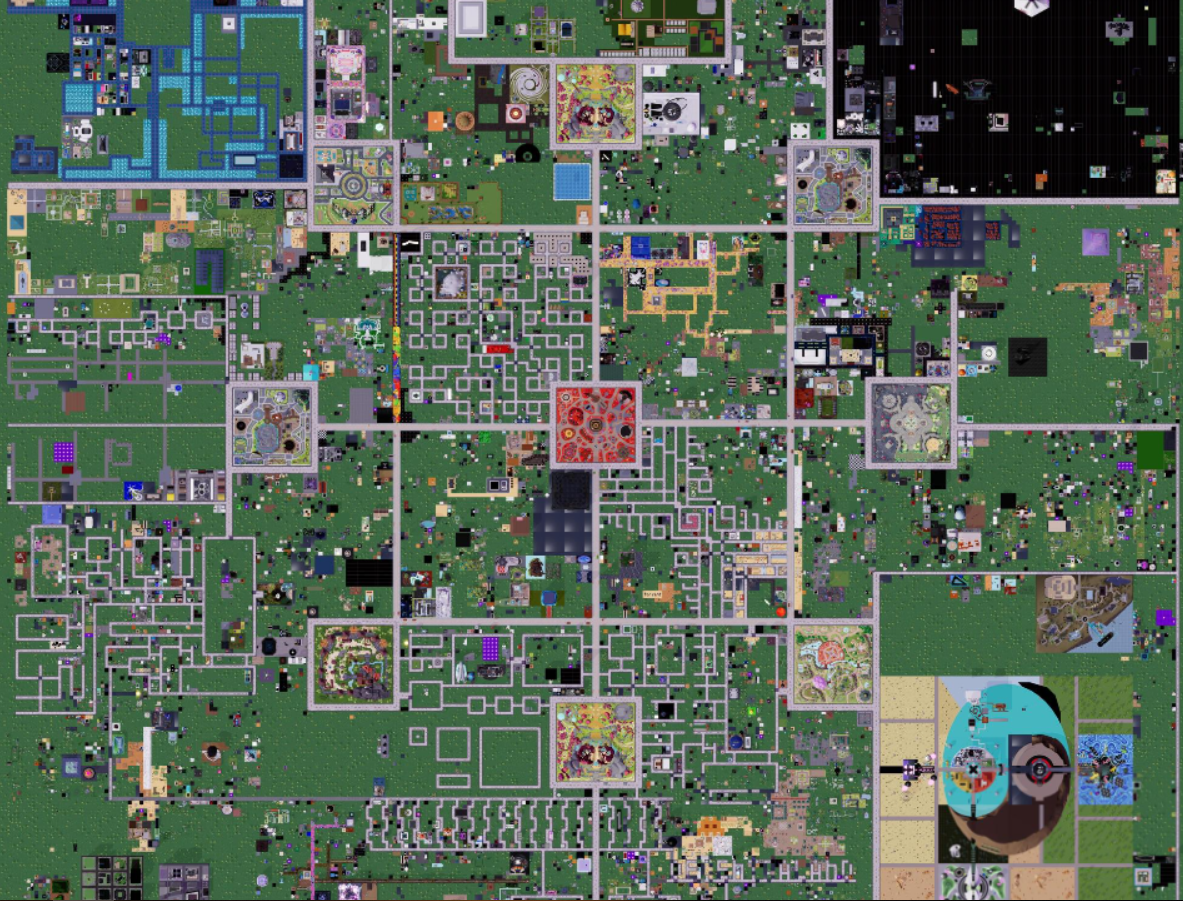
\includegraphics[width=0.8\textwidth]{dcl_map.png}
  \caption{Top view of Decentraland's map \cite{genesisCity}}
  \label{fig:dcl_map}
\end{figure}

The Decentraland DAO\cite{DCLDAO} is the decision-making tool for digital assets holders in Decentraland's virtual world. Through votes in the DAO, the community can issue grants and make changes to the lists of banned names, POIs, and catalyst nodes. The DAO also controls the \gls{LAND} and \gls{ESTATE} smart contracts.

These proposals, the votes submitted, and final results are all stored in IPFS via Snapshot, a gas-less voting client. Approved proposals with binding actions are enacted on the Ethereum blockchain by a committee by means of a multi-sig wallet. This committee is overseen by the Security Advisory Board (SAB), another multisig with trusted key holders. This Committee was voted into place by the community in the previous release of the DAO.

\chapter{Methodology}
\section{Problem}
As already mentioned in section \ref{dcl}, Decentraland is open source and community driven. Based on this, where many actors are involved in decision making, it is essential to have as much information as possible about the status of the project in order to make informed decisions.

So far there was no tool or solution that could publicly provide information to everyone about the state of the DAO treasury and the different assets of the community. Of course the information was and still is available since the blockchain is public, but not everyone has the time or knowledge to collect such data and analyze it.

Therefore, in summary, there was a need to develop a tool that would provide information publicly on the state of the DAO's treasury and the different assets of the community to enable informed decision making. \\

To begin designing the solution, three main sources were considered: \\

First, the Decentraland community. It is necessary to understand the current needs to be able to propose a solution to the problem, that is why it was taken as main input the requests of the users through conversations and interviews. \\

The next was the team that maintains the DAO platform, known as DAO Squad. From them were obtained the technical requirements needed to carry out the design of the tool and the implementation path. \\

Lastly, the Data team from the Decentraland foundation. Once all the information was obtained, it is necessary to make sense of it through charts and analytics, which is why the support of this team was provided to represent all the valuable information in the best possible way.

\section{Methods\label{methods}}
After reviewing the community's requests, it was determined that the goal of this project must be about collecting and processing Decentraland's public data and making it available to stakeholders in a consumable format. The scope includes:

\begin{itemize}
  \item \textbf{Accounting:} Tracking different streams such as
  \begin{itemize}
    \item Income
    \item Expenses
    \item Revenue
    \item Balance
  \end{itemize}
  \item \textbf{Market:} Sizing transacted value in the world and liquidity
  \begin{itemize}
    \item Tracking sales data
    \item DAO and Creators revenue
    \item Estimation of economy size
    \item Defining health indicators
  \end{itemize}
  \item \textbf{Operations:} Defining business unit performance metrics
  \begin{itemize}
    \item Teams Performance
    \item Execution times, operative expenses, etc.
    \item Does any team need to shrink or expand?
  \end{itemize}
\end{itemize}

\subsection{Requirements}
For the solution of this problem, the following requirements were mandatory:
\begin{enumerate}
  \item It must be possible to visualize the general state of the DAO's treasury and the different assets of the community.
  \item It must be possible to visualize metrics to be able to make decisions.
  \item Data collection must be from public sources.
  \item The data collection scripts must be open source.
  \item Both the information collected and the metrics performed must be accessible to anyone.
\end{enumerate}

\subsection{Data collection sources}
\subsubsection{IPFS}
The \ac{IPFS} \cite{ipfs} is a protocol, hypermedia and file sharing peer-to-peer network for storing and sharing data in a distributed file system. IPFS uses content-addressing to uniquely identify each file in a global namespace connecting IPFS hosts. It can among others replace the location based hypermedia server protocols http and https to distribute the World Wide Web.

IPFS allows users to host and receive content in a manner similar to BitTorrent. As opposed to a centrally located server, IPFS is built around a decentralized system of user-operators who hold a portion of the overall data, creating a resilient system of file storage and sharing. Any user in the network can serve a file by its content address, and other peers in the network can find and request that content from any node who has it using a \ac{DHT}.

In contrast to BitTorrent, IPFS aims to create a single global network. This means that if two users publish a block of data with the same hash, the peers downloading the content from "user 1" will also exchange data with the ones downloading it from "user 2". IPFS aims to replace protocols used for static webpage delivery by using gateways which are accessible with HTTP. Users may choose not to install an IPFS client on their device and instead use a public gateway.

\subsubsection{Infura}
Infura\cite{infura} is a blockchain development suite that provides application programming interfaces (APIs) and developer tools. It provides fast and reliable access to the Ethereum network to enable developers to build software and Web3 applications that scale to meet user demand.
As an Infrastructure-as-a-Service (IaaS) and Web3 backend infrastructure provider, it offers documentation and resources to help developers build decentralized applications (dApps) quickly. This is achieved by reducing the time spent building infrastructure from scratch. Infura offers enterprise-ready infrastructure using a distributed cloud-hosted network of nodes. This removes much of the friction associated with the development and ownership of proprietary computing and storage facilities. 

The Infura Ethereum API provides developers with easy-to-access Ethereum-based infrastructure to build decentralized applications. Using it, builders can connect applications in just a few seconds using a single line of code. This makes it simple to take advantage of fast, highly available Ethereum infrastructure. 

\begin{figure}[H]
  \centering
  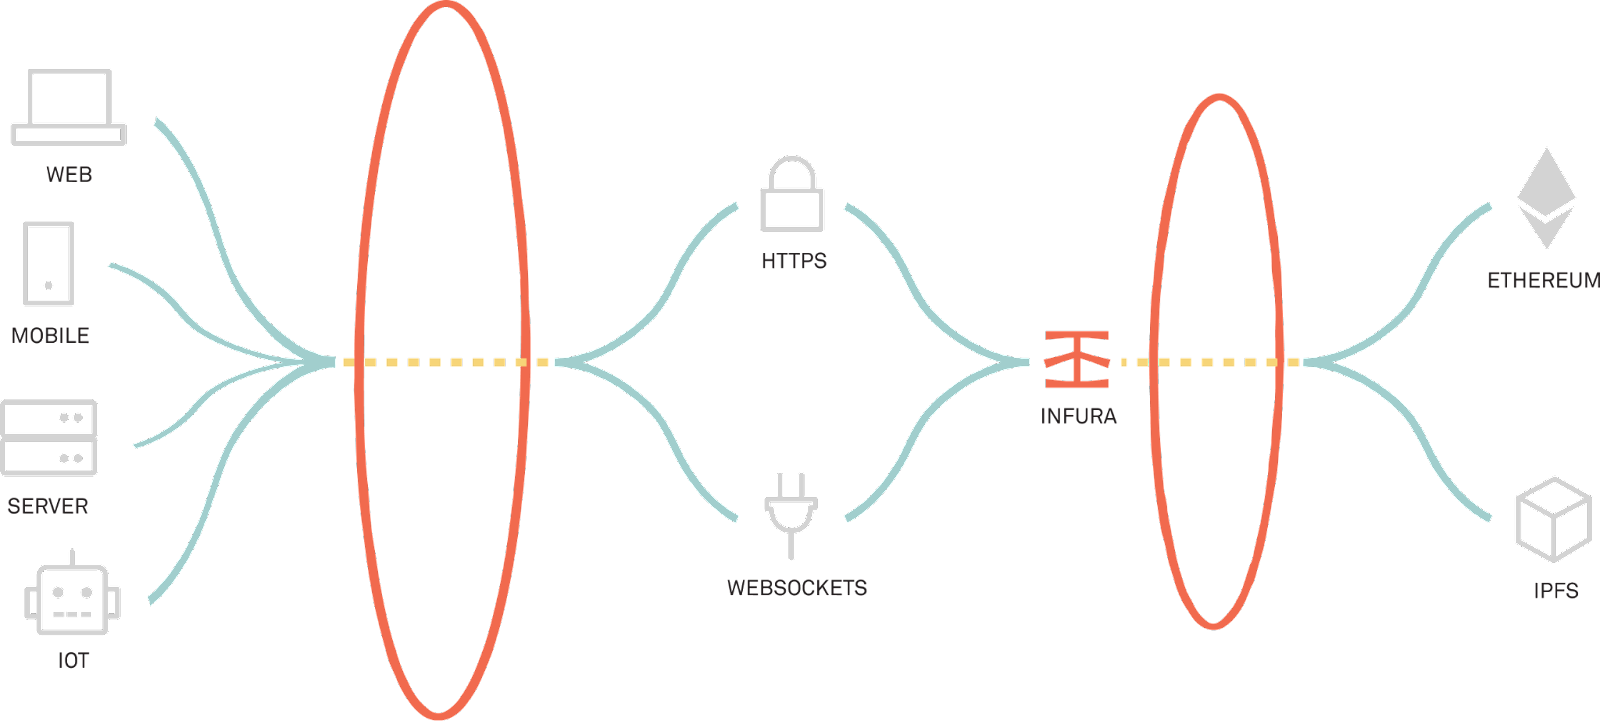
\includegraphics[width=\textwidth]{infura.png}
  \caption{Diagram of information flow through Infura \cite{infura}}
  \label{fig:infura}
\end{figure}

\subsubsection{Snapshot}
Snapshot\cite{snapshot} is a decentralized voting system. It provides flexibility on how voting power is calculated for a vote. It supports various voting types to cater to the needs of organizations. Creating proposals and voting on Snapshot is user-friendly and does not cost gas as the process is performed off-chain.
In short, Snapshot is an off-chain gasless multi-governance client with easy to verify and hard to contest results.

Its key features are: \\
\begin{itemize}
  \item Free (gasless) to create proposals and vote on them
  \item Votes are signed messages easily verifiable online
  \item Multiple voting systems - Single choice, Approval voting, Quadratic voting, and more
  \item Flexible voting strategies to calculate voting results - vote with ERC20s, NFTs, other contracts, and more
  \item Fully open-source with MIT license
\end{itemize}

\subsubsection{Covalent}
Covalent\cite{covalent} is a multi-chain unified application programming interface that brings visibility to billions of data points for multiple blockchains. As an indexing querying solution for blockchains, the platform offers a diverse range of actionable insights that enable developers to optimize the allocation of resources, bringing greater utility to decentralized applications using a single, unified API.

Covalent collates millions of data points from different organizations. Rather than searching for data from multiple locations on multiple blockchains, the network provides a one-stop-shop for high-quality multi-chain data.

This is made possible by aggregating various data feeds from nodes on different blockchains. The Covalent API then facilitates the distribution of customized data feeds to suit the individual needs of users. This data can be broad or specific, depending on the application. For example, the API can provide both the historical and current performance of digital assets. This could be for a small handful of assets or to analyze the entire crypto market. Plus, when data is requested, it is returned quickly in a uniform, consistent manner. Regardless of how many blockchains are queried, all relevant data is presented in a single API.

\chapter{Solution}
For the implementation of such tool that meets the requirements mentioned in section \ref{methods} it was decided, first of all, to create a public repository\footnote{\url{https://github.com/Decentraland-DAO/transparency}} within the Decentraland DAO organization where the code of the scripts with their respective version history will be stored. In this way, the tool is auditable by anyone who is willing to do so.

Since data must be collected every day and different sources must be consumed, Node.js was chosen for the backend of the project as it is easily configurable to run periodically in a GitHub Action\footnote{\url{https://github.com/actions/setup-node}}. As for the programming language chosen, Typescript was used due to the versatility it offers and, naturally, for the typing - since it is very useful when working with data. The collected information is available in two widely used formats: \textbf{CSV} \& \textbf{JSON}. The first one is very useful for data analysis and the second one to be consumed by other applications.

Finally, Google Data Studio\footnote{\url{https://datastudio.google.com/u/0/reporting/fca13118-c18d-4e68-9582-ad46d2dd5ce9/page/p_nlc90z86rc}} is used to visualize the metrics, which uses as input the information from the CSVs collected with the scripts (previously uploaded to a Google spreadsheet). This allows the community to have a simple way to visualize metrics that can be easily shared with other people.

\subsection{From data to metrics}

\chapter{Discussion}
\toComplete

\chapter{Conclussion}
\toComplete

\chapter{Summary}
\toComplete

\chapter{Lists}
\toComplete

\chapter{Glossary}
% \glossarysection
\printnoidxglossaries

\chapter{Appendix (optional)}
\toComplete

%
% Hier beginnen die Verzeichnisse.
%
\clearpage
\printbibliography
\clearpage
% Das Abbildungsverzeichnis
\listoffigures
\clearpage

% Das Tabellenverzeichnis
\listoftables
\clearpage

% Das Quellcodeverzeichnis
\listofcode
\clearpage

\phantomsection
\addcontentsline{toc}{chapter}{\listacroname}
\chapter*{\listacroname}
\begin{acronym}
    \acro{Crypto}{Cryptocurrency}
    \acro{Dapp}{Decentralized App}
    \acro{DAO}{Decentralized Autonomous Organization}
    \acro{NFT}{Non-Fungible Token}
    \acro{PoW}{Proof-of-Work}
    \acro{PoS}{Proof-of-Stake}
    \acro{VR}{Virtual Reality}
    \acro{AR}{Augmented Reality}
    \acro{IPFS}{InterPlanetary File System}
    \acro{DHT}{Distributed Hash Table}
\end{acronym}

%
% Hier beginnt der Anhang.
%
\clearpage
\appendix
\end{document}
